\section{Dataset Design}
\label{sec:design}

\subsection{Design Objectives}
\label{ssec:design_objectives}

The design of \lucid{} was guided by five overarching principles derived from
an analysis of gaps in the existing literature (Section~\ref{sec:related_work}):

\begin{enumerate}[leftmargin=2em, noitemsep, label=\textbf{P\arabic*.}]
  \item \textbf{Causal Completeness.} Each scenario must be annotated with a
        structured causal chain that links observable events (\eg{} a pedestrian
        stepping off a curb) to driving decisions (\eg{} emergency braking),
        enabling models to learn and explain causal event flows.
  \item \textbf{Counterfactual Coverage.} Each causal QA pair must be accompanied
        by at least one counterfactual alternative that perturbs a key causal
        variable and asks for the predicted outcome, stimulating reasoning beyond
        pattern recall.
  \item \textbf{Environmental Robustness.} Data must span diverse weather conditions,
        lighting states, geographic regions, and time-of-day settings to prevent
        distribution bias toward ideal conditions.
  \item \textbf{Multi-agent Grounding.} Annotations must capture interactions among
        multiple traffic participants (\eg{} ego vehicle, pedestrians, cyclists, other
        vehicles) and represent their intentions and interactions in language.
  \item \textbf{Benchmark Tractability.} Tasks must be defined with clear input/output
        formats, automated metrics, and reproducible evaluation protocols to enable
        objective comparison across models.
\end{enumerate}

\subsection{Scenario Taxonomy}
\label{ssec:scenario_taxonomy}

We define five top-level scenario categories based on traffic complexity, road type,
and the nature of driving decisions involved.

\begin{itemize}[leftmargin=2em, noitemsep]
  \item \textbf{Category A --- Urban Intersections (3,847 scenarios, 29.9\%)}: Signalised
        and unsignalised intersections, roundabouts, and complex multi-lane crossings
        in urban environments. These scenarios demand integration of traffic signal state,
        pedestrian crossing predictions, and multi-agent gap acceptance decisions.
  \item \textbf{Category B --- Highway Merging and Lane Changes (2,156 scenarios, 16.8\%)}:
        High-speed merging from on-ramps, lane-change sequences, and cooperative
        car-following behaviours. Causal chains frequently involve velocity estimation,
        gap acceptance, and predictive trajectory modelling.
  \item \textbf{Category C --- Pedestrian-dense Zones (2,891 scenarios, 22.5\%)}: School
        zones, market streets, crosswalks, and transit hubs. Rich in yielding, stopping,
        and prediction-under-uncertainty decisions.
  \item \textbf{Category D --- Long-tail Edge Cases (2,318 scenarios, 18.0\%)}: Rare but
        high-impact events: sudden object falls, emergency vehicle approaches, unexpected
        road obstacles, and sensor-degrading conditions. Long-tail coverage is critical for
        safety validation of LLM-based planners.
  \item \textbf{Category E --- Parking and Low-speed Manoeuvres (1,635 scenarios, 12.7\%)}:
        Parking lot navigation, reversing, U-turns, and low-speed pedestrian co-navigation.
        These scenarios emphasise spatial reasoning and close-quarters planning.
\end{itemize}

\subsection{Annotation Schema}
\label{ssec:annotation_schema}

\lucid{} introduces a \emph{hierarchical annotation schema} operating at four levels:

\paragraph{Level 1 --- Scene Description.}
A free-form natural language description of the overall driving scene, including
road geometry, weather, visible agents, and any salient objects. Scene descriptions
are collected per key frame (\ie{} every 30 frames, at 0.33 Hz).

\paragraph{Level 2 --- Agent Intention Labels.}
For each detected traffic participant, annotators assign an intention label drawn
from a closed vocabulary of 27 motion primitives (\eg{} \emph{pedestrian:about-to-cross},
\emph{vehicle:cutting-in}, \emph{cyclist:decelerating}). Agent labels are provided at
the object track level and linked to the scene graph for each keyframe.

\paragraph{Level 3 --- Causal Chain QA Pairs.}
The core novel annotation type. Each causal chain is structured as a directed
graph $\mathcal{G} = (V, E)$ where nodes $V$ represent driving events and directed
edges $E$ represent causal dependencies. From each graph, we derive a set of
\emph{causal QA pairs} following the template:
\begin{quote}
  \textit{``[Observation]: [event]. [Cause question]: Why did this occur?
  [Answer]: Because [causal antecedent].''} \\[4pt]
  \eg{} \textit{``The ego vehicle slowed from 50~km/h to 15~km/h.
  Why? Because a child ran into the crosswalk from the right, and the traffic
  signal had just turned amber.''} 
\end{quote}
On average, each scenario contains 24.3 causal QA pairs (min 4, max 187).

\paragraph{Level 4 --- Counterfactual QA Pairs.}
Each causal QA pair is accompanied by one or more counterfactual variants that
alter a key causal variable and elicit a prediction about the modified outcome:
\begin{quote}
  \textit{``[Counterfactual premise]: What would have happened if [modified condition]?
  [Counterfactual answer]: If [modified condition], then [predicted outcome].''} \\[4pt]
  \eg{} \textit{``What would have happened if the child had not entered the crosswalk?
  The vehicle would have maintained its speed and cleared the intersection without braking.''} 
\end{quote}
Counterfactual pairs are validated by a domain expert reviewer to ensure physical
plausibility. Each scenario contains 15.4 counterfactual pairs on average.

\paragraph{Level 5 --- Risk Assessment and Planning Instructions.}
Each scenario is annotated with (a) a structured risk matrix classifying hazard
type, severity, and probability, accompanied by a natural-language explanation;
and (b) a set of natural-language planning instructions specifying the optimal
manoeuvre sequence (\eg{} \textit{``Apply moderate braking, maintain a 3-second
following distance, and prepare for a right-lane merge after the intersection''}).

\begin{figure}[t]
  \centering
  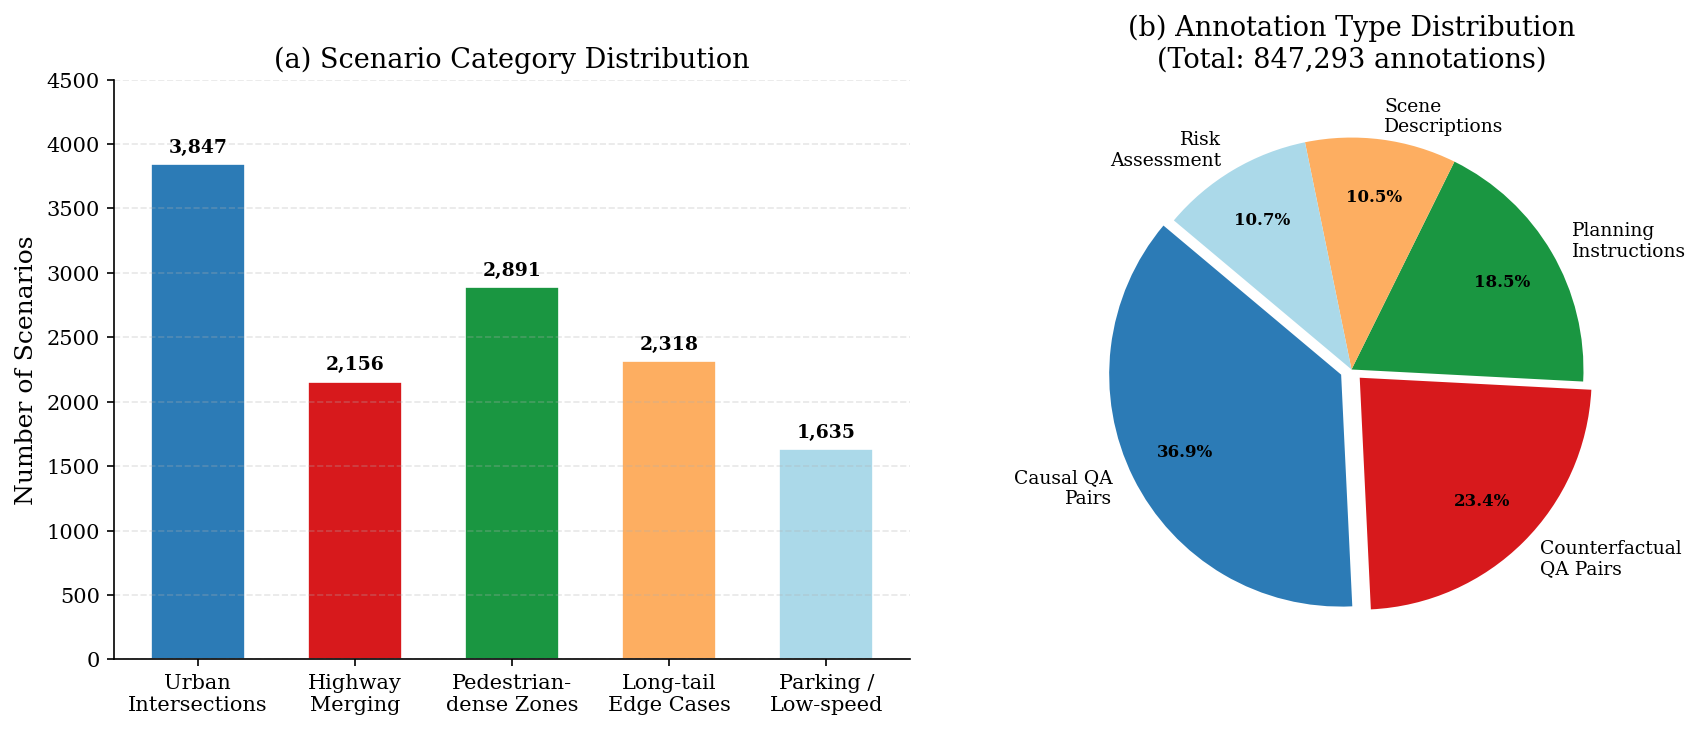
\includegraphics[width=\linewidth]{figures/scenario_and_annotation.png}
  \caption{Left: distribution of the 12,847 scenarios across the five scenario categories.
  Right: distribution of the 847,293 language annotations across the five annotation types.
  Causal and counterfactual QA pairs together constitute 60.7\% of all annotations,
  representing the novel contribution of \lucid{}.}
  \label{fig:distributions}
\end{figure}

\subsection{Causal Chain Model}
\label{ssec:causal_model}

We formalise the causal structure of each scenario using a \emph{Causal Event Graph}
(CEG), inspired by Pearl's do-calculus~\cite{pearl2009causality} and adapted for
time-stamped driving events. A CEG is a directed acyclic graph (DAG) $\mathcal{G} = (V, E, T)$
where:
\begin{itemize}[leftmargin=2em, noitemsep]
  \item $V$ is a finite set of \emph{event nodes}, each representing a discrete
        observable occurrence (\eg{} ``vehicle enters ego lane at $t=4.2s$'').
  \item $E \subseteq V \times V$ is a set of directed causal edges, where $(u, v) \in E$
        denotes that event $u$ causally contributes to event $v$.
  \item $T: V \to \mathbb{R}^+$ is a timestamp function mapping each event to its
        occurrence time in the scenario.
\end{itemize}
Counterfactual reasoning is operationalised via \emph{graph surgery}: a counterfactual
premise corresponds to removing or modifying the value of a specific node $v^* \in V$
and querying the downstream impact on dependent nodes.

\subsection{Counterfactual Generation Methodology}
\label{ssec:counterfactual_gen}

Counterfactual premises were generated through a combination of (1) manual creation
by domain-expert annotators (for safety-critical events) and (2) semi-automatic
generation using a guided prompting protocol with a large language model followed
by mandatory human validation. The LLM-assisted generation used structured prompts
that specified the causal event to perturb and required annotators to accept,
reject, or revise each generated counterfactual before it was admitted to the dataset.
This hybrid approach achieved a productivity gain of $3.2\times$ over fully manual
counterfactual authoring while maintaining human-verified quality standards.
